
{\chapter{Characterization of cancer transcriptomics under drug perturbations in TNBC-PDX}

}
 \label{ch:Chapter5}
 \section{Motivation}

In spite of advanced technologies and treatment, triple negative breast cancer still facing the problems of tumor recurrence and drug resistance.
For any given difference between the types of drug resistance, for example, the expression of a particular gene, it is assumed that differences arise deterministically or probabilistically in the configuration of transcription factors regulating the genes in the tumors. Cancer cells in distinct cell- states often exhibit important differences in functional properties depending on the which genes are turned on and off resulting in sensitive or resistant phenotype.

The most challenging analysis is to differentiate whether the change in gene expression leading to change in cellular state is stochastic\cite{raj2008nature} and random or its deterministic to produce the same output under similar environment.
Cancer cells in distinct cell- states often exhibit important differences in functional properties depending on which genes are turned on and off resulting in sensitive  or resistant phenotype.
Previously it is shown that unique cells within a population can exhibit fluctuations in expression of a group of genes, that could predict distinct phenotypes \cite{shaffer2019memory}.


\begin{figure}
\centering
  
  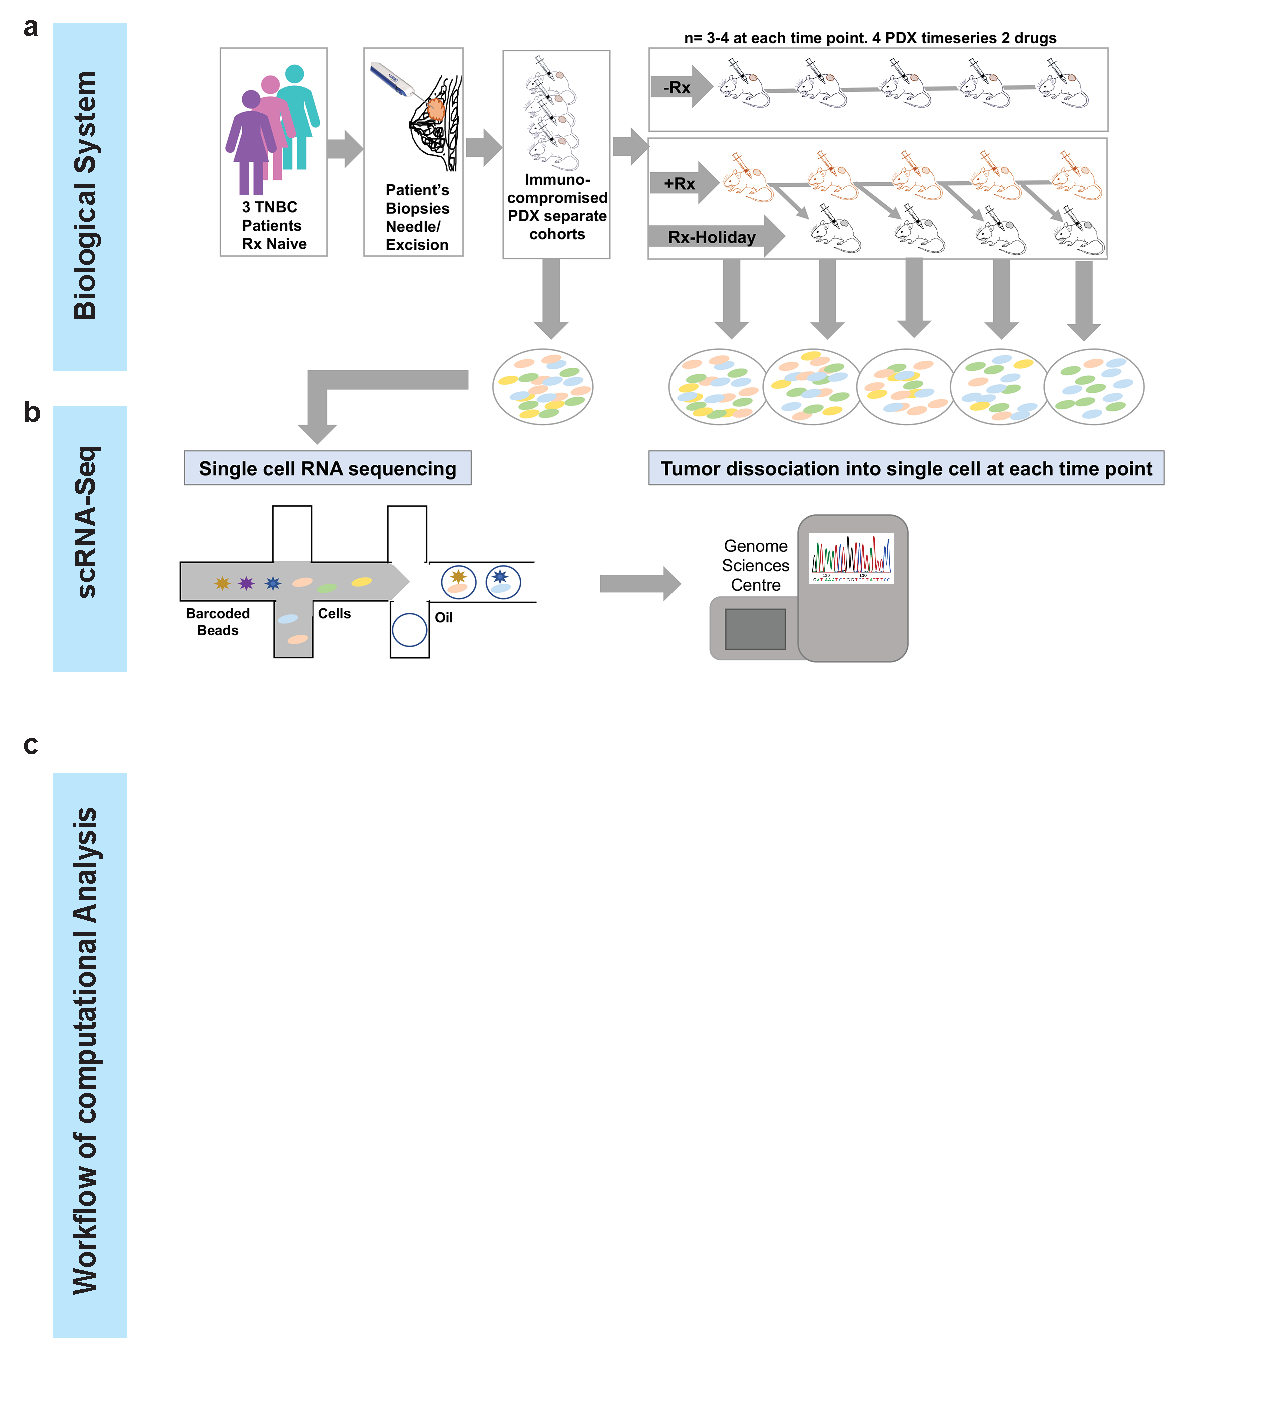
\includegraphics[width=\textwidth]{Figures/fig1schematicsoverview.pdf}
	
\caption[Schematic overview of experimental design and analysis pipeline.]
	{\small
	\textbf{Need to update: Schematic overview of experimental design and analysis pipeline.}
	   Upper panel shows biological systems used to acquire single cell RNA sequencing data. The time point tumors are similar to DLP+ samples in Chapter 4. After applying filters and normalization, various packages are used for analysis as mentioned in the lower half of the schematics.
	 
	}
	\label{fig:fig1schematicsoverview}
\end{figure}


Un-like genomic clones that could get selected in resistant phenotype \cite{salehi2020single}, we still are not clear whether the cell-states are acquainted for this kind of behaviour or the selected states are pre-existing in the cancer population and under continues pressure shows obvious dynamics or there is a transition from one state to another that ultimately gets selected over time. Because of difficulty to analyse longitudinal patient's samples for single cell gene expression and lack of multiple longitudinal pre-clinical breast cancer models, these questions remains unexplored. Here we set to examine three breast cancer patient derived xenografts (PDX) that were serially challenged for around 4-5 cycles with the drug until they started showing less response to the treatment. We wanted to understand the magnitude of fluctuations in gene expression from sensitive to resistant phenotype.


 \section{Synopsis}
   From the previous chapter we know that the population changes with the tumor growth from one passage to another with and without the drugs. We see the shifts in the clones and some clones get selected and others disappear.
   Now in this chapter, first of all we sought to determine whether under neutral conditions when there is no drug pressure what proportion of the transcriptomes might be copy number driven just due to the natural evolution of the copy number clones. This allows us to understand the stability of the gene expression in our timeseries models in the absence of drugs.
   Next, we explored that on drug being introduced into the system, how much of the drug induced change in expression is dependent on the copy number and which are independent.




\section{Results}


\subsection{Clone-specific genotypes underpin clone-specific gene expression programs}
We profiled the impact of clone specific gene expression changes as a higher order representation of phenotypic properties. We tested if the genotypes of high fitness clones exhibited changes in their transcriptional program, with scRNAseq performed on matched aliquots of samples sequenced using DLP+ on the serially passaged triple-negative breast cancer patient-derived xenografts from Chapter 4 as substrates \textbf{(\autoref{fig:treatedtimeseriesmanuscript)}}.

\subsubsection{Copy number change and scRNAseq expression revealed legitimate correlation across PDX timeseries}
  In our approach, we assume clones are defined through grouped cell subsets which share to a first approximation similar genomic copy number structure (e.g., through phylogenetic reconstruction or dimensionality reduction) \cite{laks2019clonal}. Based on this relationship we applied
  \texttt{clonealign} approach \cite{campbell2019clonealign} to reveal clone-specific phenotypic properties across all samples.
  Each point is taken as the proportion of DLP cells in a clone horizontal axis versus the proportion of the scRNAseq cells in the same clone. The  correlation for all clones were then calculated by using Pearson correlation coefficient formula. The heat maps of SA609 TNBC PDX \textbf{(\autoref{fig:UnRxseries} h)} and SA535 TNBC PDX \textbf{(\autoref{fig:SA535analysis} a,e)} exhibit more complex heterogeneity at copy number space along with structural genomic rearrangements as compared to SA1035 TNBC PDX \textbf{(\autoref{fig:SA1035Rxnew} a, e)}. Our results showed DLP+ and \texttt{clonealign} clone abundance measures were positively correlated across all libraries \textbf{\autoref{fig:fig2_clonealignembeddings.pdf} a, d, g}. Importantly, SA535 TNBC treated with cisplatin present the high confidence correlation with Pearson correlation 0.97 (p$<$0.001), followed by its CX-5461 treated series, presenting Pearson correlation of 0.94 (p$<$0.001) \textbf{\autoref{fig:fig2_clonealignembeddings.pdf} g}. However, SA609 PDX timeseries samples present a Pearson correlation coefficient of 0.94 (p$<$0.001) \textbf{(\autoref{fig:fig2_clonealignembeddings.pdf} a)} and SA1035 PDX with Pearson correlation of 0.78 (p$<$0.001) \textbf{(\autoref{fig:fig2_clonealignembeddings.pdf} d)}.
  
  

\begin{figure}
\centering
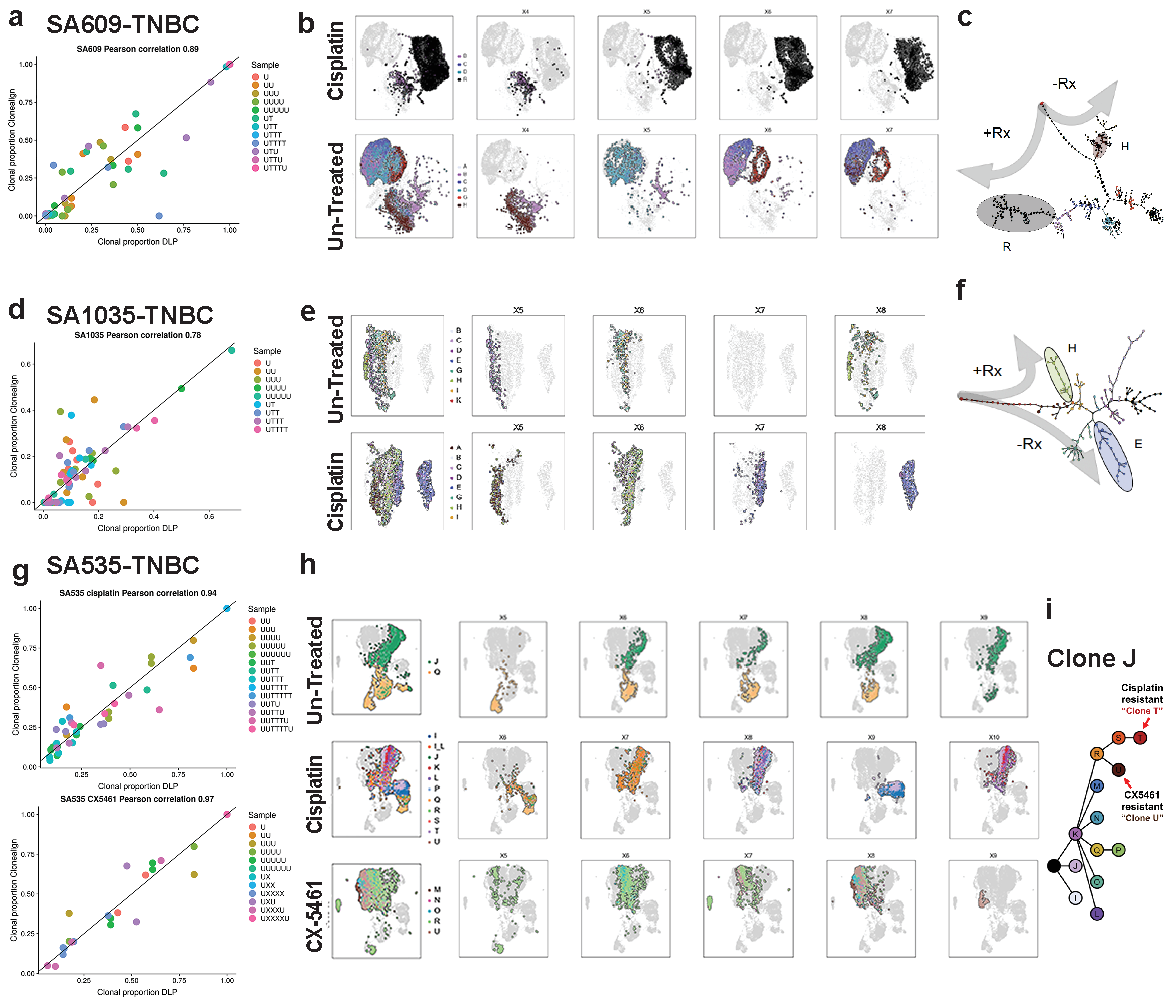
\includegraphics[width=\textwidth]{Figures/fig2_clonealignembeddings.pdf}
	
\caption[Gene expression impacts of clone-specific copy number profiles]
	{\small
	\textbf{Gene expression impacts of clone-specific copy number profiles.}
	   \textbf{(a)} \texttt{clonealign} clonal proportions vs DLP+ clonal proportions of SA609 PDX timeseries samples indicating positive correlation (Pearson correlation from 0.89).
	    \textbf{(b)} Low dimensional \ac{UMAP} embeddings of matching scRNAseq libraries across the SA609 TNBC timeseries. Left top and bottom panels show treated and untreated complete embedding annotated with clonealign assignments and right all panels show the density of cell clusters over the timeseries X4-X7.
	     \textbf{(c)} Phylogeny of SA609 taken from previous chapter to recall emerged clones with or without drug. 
	     \textbf{(d)} Same like \textbf{(a)} but for SA1035 PDX and Pearson correlation is 0.78. \textbf{(e)} Same like \textbf{(b)} but for SA1035 starting from X5-X8. \textbf{(f)} Same like \textbf{c} but for SA1035. \textbf{(g)} Same like \textbf{a} but for SA535 PDX and Pearson correlation is 0.94 for cisplatin treated and 0.97 with CX-5461 treated. \textbf{(h)} Same like \textbf{b} but for SA535 starting from X5-X9, X10.
	}
	\label{fig:fig2_clonealignembeddings.pdf}
\end{figure}



\subsubsection{Single cell RNAseq clusters exhibit a dynamic pattern of global expression over time which tracked with clone assignments}
Next, we visualized the data using UMAP \cite{becht2019dimensionality}, dimensionality reduction method, to aggregate cells into treated and untreated subpopulations while retaining the relationship between subpopulations. scRNAseq embeddings displayed a dynamic pattern of global expression over time with and without treatment, which tracked with clone assignments indicating co-variation of transcriptional properties with clonal abundance \textbf{\autoref{fig:fig2_clonealignembeddings.pdf}}. UMAP Visualization of clusters identified clone H clusters in untreated setting and clone R clusters, in the cisplatin treated series of SA609 TNBC PDX, purified over time matching their genomically defined counterparts \textbf{(\autoref{fig:fig2_clonealignembeddings.pdf} b)}. Similarly, clone E in untreated and clone H in treated timeseries of SA1035  \textbf{(\autoref{fig:fig2_clonealignembeddings.pdf} e)}, clustered uniquely at the later time points. \textbf{\autoref{fig:fig2_clonealignembeddings.pdf} c, f} reminding the clones emerging with and without treatment through the phylogeny of DLP+ from chapter 4, in SA609 and SA1035, respectively.  SA535 TNBC PDX all three arms of untreated, treated with cisplatin and CX-5461, exhibited aggregation of similar patterns of clusters that favours emerging of genomic clones in their respective series. Clone J, in untreated control timeseries \textbf{(\autoref{fig:fig2_clonealignembeddings.pdf} h, upper panel)}, clone T, in cisplatin timeseries 


\subsection{Copy number dependent in-cis and trans regulated gene expression rates in scRNAseq data set}



\begin{figure}
\centering
  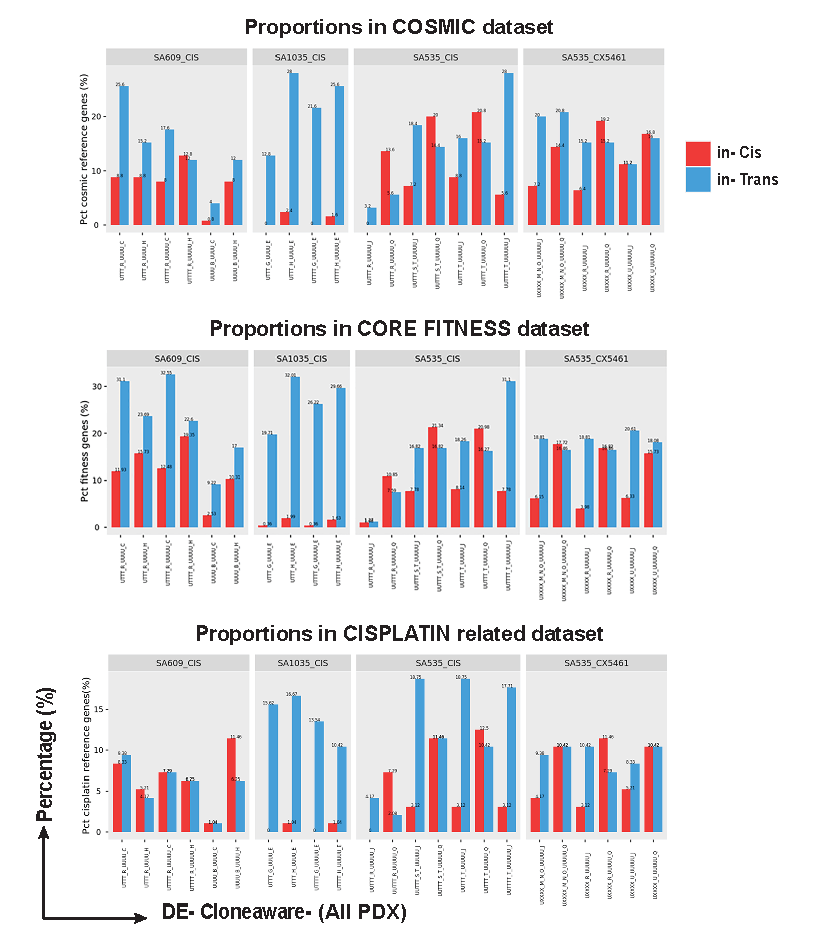
\includegraphics[width=\textwidth]{Figures/fig3_In_cispercentage.pdf}
	
\caption[Proportion of in-cis and in-trans regulated gene expression in scRNAseq data]
	{\small
	\textbf{Proportion of cis and trans regulated gene expression in scRNAseq data.}
	   Horizontal axis shows differential expression between two selected clones from all the three PDX treated and un-treated timeseries. Vertical axis gives percentage presence of genes in-cis or in trans. red bars represent in-cis and blue bars represent in -trans regulated gene expression.
	   \textbf{(Upper)} This graph gives us percentage of genes by looking into the gene data set from COSMIC cancer gene dataset \cite{vogelstein2013cancer} that corresponds to our clone aware \ac{DE}.
	    \textbf{(Middle)} same like upper plot but looking into CORE FITNESS data set \cite{behan2019prioritization}.
	     \textbf{(Lower)} Same like above but looking into cisplatin related gene list curated from literature.
	    
	}
	\label{fig:fig3_In_cispercentage}
\end{figure}



\subsection{Differential expression  analysis of resistant and sensitive clones}




\begin{figure}
\centering
  \includegraphics[width=\textwidth]{Figures/fig4_Volcanotrackplots2.pdf}
\caption[DE of resistant and sensitive clonealign defined clones]
	{\small
	\textbf{Differential expression of resistant and sensitive clones.}
	\textbf{(a)} Volcano plot from SA609 -log10(FDR) plotted against log2 fold change of pairwise differential gene expression between resistant and sensitive clones. Manhattan plot (genome-wide view) of differential gene expression between pairs of clones, R vs H corresponding to change in gene expression (Right).
	    \textbf{(b)} Same like \textbf{a} but in SA1035 and comparing between pairs of clones, H vs E. 
	     \textbf{(c)} Same like \textbf{a} but in SA535 (cisplatin) and comparing between pairs of clones, S\_T vs J. 
	     \textbf{(d)} Same like \textbf{a} but in SA535 (CX-5461) and comparing between pairs of clones, U vs J.
	   \textbf{(e)} Barplot showing copy number driven percentage of in cis or in trans up and down regulation of genes.
	   \textbf{(f)} Barplots showing summary of total in cis and in trans proportion in the whole data set.
	     \textbf{(g-j)} Manhattan plot (genome-wide view) of differential gene expression between pairs of clones, from \textbf{a, b, c, d}. }
	\label{fig:fig4_Volcanotrackplots2}
\end{figure}




\begin{figure}
\centering
  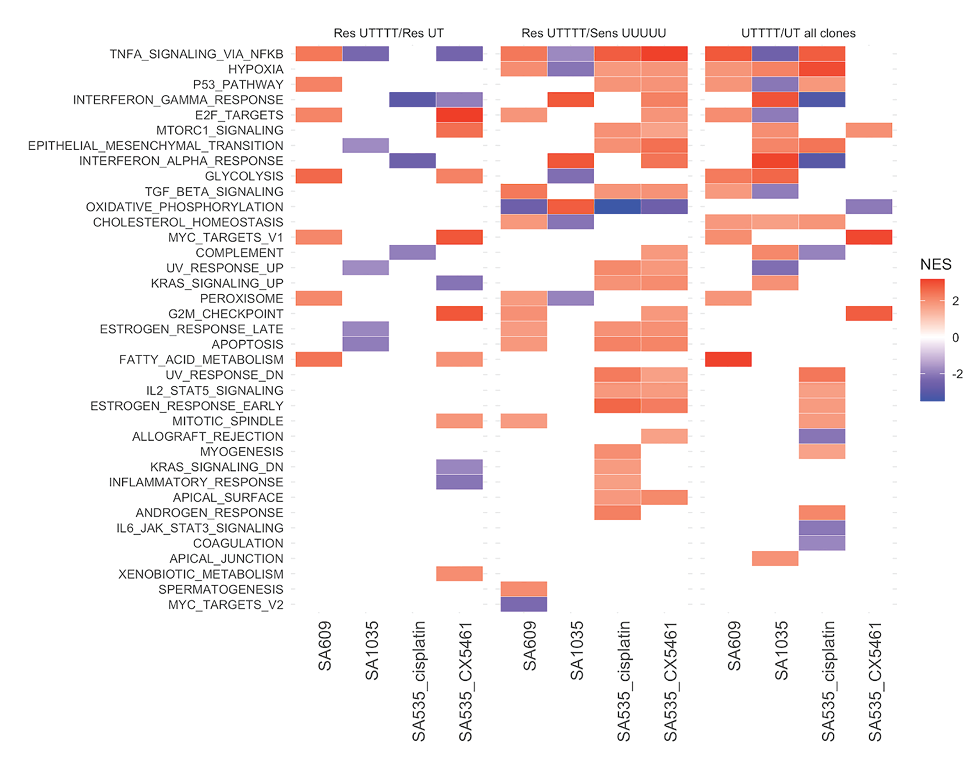
\includegraphics[width=\textwidth]{Figures/fig5pathwaysnetwork.pdf}
\caption[Pathways enrichment analysis of PDX timeseries]
	{\small
	\textbf{Pathways enrichment analysis of PDX timeseries.}
	 Vertical axis on the left enlisting the pathways involved under various conditions in timeseries PDXs. Left panel comparing resistant clone versus clone exposed to only one cycle of drug. Middle panel comparing resistant versus sensitive clone in all PDXs. Right panel comparing last treated timepoint as a whole with first treated timepoint. Horizontal axis is showing the names of PDXs.
	}
	\label{fig:fig5pathwaysnetwork}
\end{figure}

\begin{figure}
\centering
  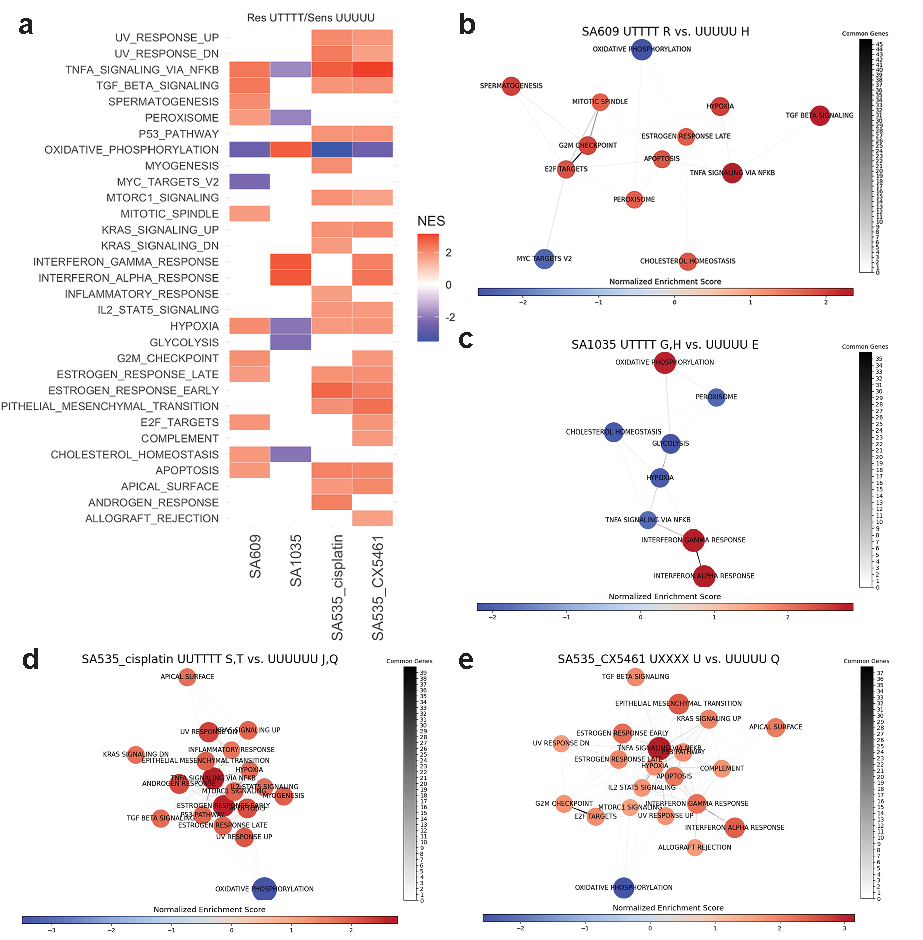
\includegraphics[width=\textwidth]{Figures/fig6resistantsensitivenetwork.pdf}
\caption[DE of resistant and sensitive clonealign defined clones]
	{\small
	\textbf{Pathway enrichment network comparing resistant and sensitive clones across timeseries PDX.}
	\textbf{(a)} Normalized enrichment score of Pathways between resistant and sensitive clone of all treated timeseries PDXs.
	    \textbf{(b)} Pathway enrichment network comparison of clone R vs clone H in SA609. Colour of grey to black lines between the pathways show strength of common genes on scale vertically drawn on right side. 
	     \textbf{(c)} Same like \textbf{a} but in SA1035  and comparing pathways between pairs of clones, G\_H vs E. 
	     \textbf{(d)} Same like \textbf{a} but in SA535 (Cisplatin) and comparing between pairs of clones, S\_T vs J\_Q.
	 \textbf{(e)} Same like \textbf{a} but in SA535 (CX-5461) and comparing between pairs of clones, U vs Q.}
	
	\label{fig:fig6resistantsensitivenetwork}
\end{figure}










\subsubsection{SA609-TNBC-FBI PDX up regulated pathways in resistant clone}


\subsubsection{SA535-TNBC-BRCA deficient PDX up regulated pathways in resistant clone}
Next we compared the emerging clone under drug pressure with the clone that could not survive the repeated drug exposures. We identified the following significantly up regulated pathways:
- Apoptosis, Epithelial mesenchymal transition, Hypoxia, mitotic spindle, MTORC1 signaling, MYC targets-V1, P53 pathway, TGF Beta signaling, TNFA signalling via NFKB, UV response up, UV response down, KRAS signaling, Angiogenesis, PI3K AKT MTOR signaling, unfolded protein response.


\subsubsection{SA1035-TNBC-APOBEC deficient PDX up regulated pathways in resistant clone}




\subsection{key Pathways and genes shared among the three TNBC PDX}




\subsection{Distinct genes monotonically increasing and decreasing with drug} 


